\documentclass[11pt]{article}
\usepackage[margin=1in]{geometry}
\usepackage{graphicx}
\usepackage{booktabs}
\usepackage{amsmath}
\usepackage{xcolor}
\usepackage{float}
\usepackage[hidelinks]{hyperref}
\usepackage{caption}
\captionsetup{font=small,labelfont=bf}
\usepackage{sectsty}
\definecolor{ohno}{HTML}{0072B2}
\definecolor{ssd}{HTML}{D55E00}
\sectionfont{\color{black!80}}
\newcommand{\ohno}{\textcolor{ohno}{\textbf{clustered cis-ohnolog}}}
\newcommand{\ssd}{\textcolor{ssd}{\textbf{clustered SSD-tandem}}}
\graphicspath{{../results/figures/}}

\title{\textbf{Chromatin architecture of clustered TF-paralog loci:\\
CTCF insulation, ATAC accessibility, and ENCODE-rE2G enhancer wiring}\\[2pt]
\large ohnolog vs.\ small-scale-duplication (tandem) clusters}
\author{Iteration 19 --- Paralogous TF project\\\small ETS P01 genomics platform}
\date{2026-07-18}

\begin{document}
\maketitle

\begin{abstract}
\noindent We profile three complementary layers of regulatory architecture over the \emph{same}
77 clustered TF-paralog loci ($47$ \ohno{}, $30$ \ssd{}) from the iteration-16 four-group
duplication catalog: \textbf{CTCF} (insulation), \textbf{ATAC-seq} (accessibility) and the new
\textbf{ENCODE-rE2G} (enhancer$\rightarrow$gene wiring). \emph{CTCF} (ENCODE GM12878
\texttt{ENCFF796WRU} and CD4 T cell \texttt{ENCFF858TLX}): bulk insulator density is
indistinguishable between groups (all $p>0.7$), and the only separating metric --- more CTCF peaks
\emph{between} the two ohnolog members --- is explained by their larger inter-member spacing.
\emph{ATAC} and \emph{E2G} (regulatory CD4 T cell / Treg, matching the project's autoimmunity
focus; \texttt{ENCFF519QMA} and \texttt{ENCFF393GIF}) reveal what the CTCF layer does not: the two
groups differ sharply in accessibility and enhancer wiring. \ssd{} paralogs live in a shared,
highly accessible regulatory neighbourhood, whereas \ohno{} paralogs --- though also clustered ---
have sparser, more independent wiring. ATAC
promoters of SSD-tandem members sit essentially on top of an accessible peak (median nearest peak
$446$~bp vs.\ $25{,}492$~bp for ohnolog; Mann--Whitney~U $p=1.8\times10^{-4}$), and E2G predicts
that SSD-tandem paralogs \emph{share the same enhancers}: a median of $10.5$ enhancer elements are
linked to \emph{both} members (vs.\ $0$ for ohnolog; $p=3.3\times10^{-5}$), and $63\%$ of
SSD-tandem pairs share $\geq 1$ enhancer vs.\ $19\%$ of ohnolog pairs. The shared-enhancer
signature reproduces in \emph{all six} lymphoid cell types tested (Treg plus five additional
ATAC-based ENCODE-rE2G sets: memory CD4, CD8, Jurkat, NK and B cells; ohnolog median $=0$ in
every one; $p$ from $1.7\times10^{-5}$ to $4.4\times10^{-3}$).
\end{abstract}

\section{Data and provenance}
\textbf{Duplication catalog (reused, not recomputed).} The two clustered classes and their locus
coordinates were taken verbatim from iteration~16 (\texttt{TF\_dup\_2x2\_classification.tsv},
\texttt{clustered\_paralogs.noKRABHOX.tsv}; hg38 / GENCODE~v45). Analysis is restricted to the
\ohno{} ($n=47$ loci) and \ssd{} ($n=30$ loci) classes; the single chrY locus (HSFY1/HSFY2) is
excluded for consistency with the CTCF baseline. Windows = cluster span $\pm$100~kb, clipped to
hg38 chromosome bounds (identical to the CTCF analysis; \texttt{clustered\_loci\_windows.pm100kb.tsv}).

\textbf{(A) CTCF insulation.} ENCODE CTCF ChIP-seq, two cell types: \texttt{ENCSR000DZN} / file
\texttt{ENCFF796WRU} (GM12878 B-lymphoblastoid, conservative-IDR narrowPeak, $44{,}217$ peaks;
constitutive reference) and \texttt{ENCSR470KCE} / file \texttt{ENCFF858TLX} (primary resting CD4
$\alpha\beta$ T cell, IDR narrowPeak, $40{,}346$ peaks; matched lineage for the Treg accessibility
data). Both GRCh38, downloaded 2026-07-18.

\textbf{(B) ATAC-seq accessibility.} ENCODE experiment \texttt{ENCSR159GFS} (ATAC-seq, biosample
CD4$^+$CD25$^+$ $\alpha\beta$ regulatory T cell / Treg), file \texttt{ENCFF519QMA} ---
\emph{IDR-thresholded peaks}, \texttt{bed narrowPeak}, GRCh38; $57{,}636$ peaks. Fed to the CTCF
pipeline scripts (\texttt{03/04/05/06}) via \texttt{-{}-subdir atac}, so the binning, per-locus,
flank and paired-promoter code is reused unchanged (in that subdir ``peaks'' denotes ATAC
accessibility peaks).

\textbf{(C) ENCODE-rE2G enhancer--gene links (the ``new E2G dataset'').} Annotation
\texttt{ENCSR759OVP} (``enhancer gene links in regulatory CD4 T cells''; multiomic ENCODE-rE2G
model combining ATAC-seq, H3K27ac, Hi-C and RNA), file \texttt{ENCFF393GIF} --- \emph{thresholded
element--gene links}, \texttt{bed3+}, GRCh38; $295{,}377$ links / $93{,}685$ unique regulatory
elements. Each row is a regulatory element $(\mathrm{chr},\mathrm{start},\mathrm{end})$ predicted to
regulate a \texttt{TargetGene}, with an ABC/rE2G \texttt{Score}, \texttt{DistanceToTSS}, per-element
ATAC accessibility (\texttt{Open}) and a class label (promoter / lncRNA / intergenic / genic).
Both files downloaded 2026-07-18 from \href{https://www.encodeproject.org}{encodeproject.org}
(provenance in \texttt{log/encode\_download.log}).

\section{Methods}
\textbf{CTCF (insulation).} Each clustered locus, extended by $\pm$100~kb, was profiled with scripts
\texttt{03/04/05/06}: per-locus CTCF peaks/kb in the window / body / flanks; observed/expected vs.\
the genome-wide CTCF rate; nearest CTCF peak to each member TSS; and the number of CTCF peaks lying
\emph{between} the two paralog members (both raw and normalized to inter-member distance). Run for
both the GM12878 and CD4 T-cell peak sets.
\textbf{ATAC (accessibility mirror).} Each locus window was profiled exactly as for CTCF: per-locus
ATAC peaks/kb in the window, locus body and flanks; observed/expected vs.\ the genome-wide ATAC
rate; a length-normalized metagene ($20$ fixed flank bins $+$ $20$ scaled body bins per side);
distance from each member TSS to the nearest ATAC peak; and peaks between the two promoters.
\textbf{E2G (script \texttt{07\_e2g\_promoters.py}).} (1) \emph{Per-locus element density}: unique
elements (deduped by coordinate) counted in the window/body/flanks, elements/kb and obs/exp vs.\ a
genome-wide baseline of $0.031$ elements/kb. (2) \emph{Gene-pair promoter wiring}: for each cluster
we collected all E2G links whose \texttt{TargetGene} is a cluster member, and counted per member the
distinct enhancer elements landing on that promoter; per pair we counted enhancer elements linked to
\emph{both} paralogs (``shared enhancers''), both genome-wide and restricted to the $\pm$100~kb
window. \textbf{Statistics.} All two-group tests are two-sided \textbf{Mann--Whitney~U},
\ohno{} vs.\ \ssd{}, reported with $U$, $p$, per-group $n$, medians and rank-biserial effect size
(\texttt{results/ctcf/atac/ctcf\_group\_comparison.tsv}, \texttt{results/e2g/e2g\_group\_comparison.tsv}).

\section{Results}

\subsection{Integrated view: three assays over one locus set}
Because all three assays were run over the identical set of clustered loci, their headline metrics
can be read side by side (Fig.~\ref{fig:integrated}, Table~\ref{tab:integrated}). They separate the
two groups in a mutually consistent way. \textbf{CTCF} places \emph{more} insulator peaks between the
two ohnolog members (median $3$ vs.\ $0$ for SSD-tandem; $p=8.9\times10^{-3}$) --- but, as shown
below, this is a consequence of ohnolog members sitting farther apart, not of denser intervening
insulation. \textbf{ATAC} shows SSD-tandem promoters essentially on top of an open-chromatin peak
(nearest ATAC peak $446$~bp vs.\ $25{,}492$~bp; $p=1.8\times10^{-4}$). \textbf{E2G} shows SSD-tandem
paralogs sharing a median of $10.5$ enhancers versus $0$ for ohnolog ($p=3.3\times10^{-5}$). The
three layers agree on a single axis: ohnolog paralog pairs are wired for regulatory
\emph{independence}, SSD-tandem pairs for \emph{co-regulation}.

\begin{figure}[H]
\centering
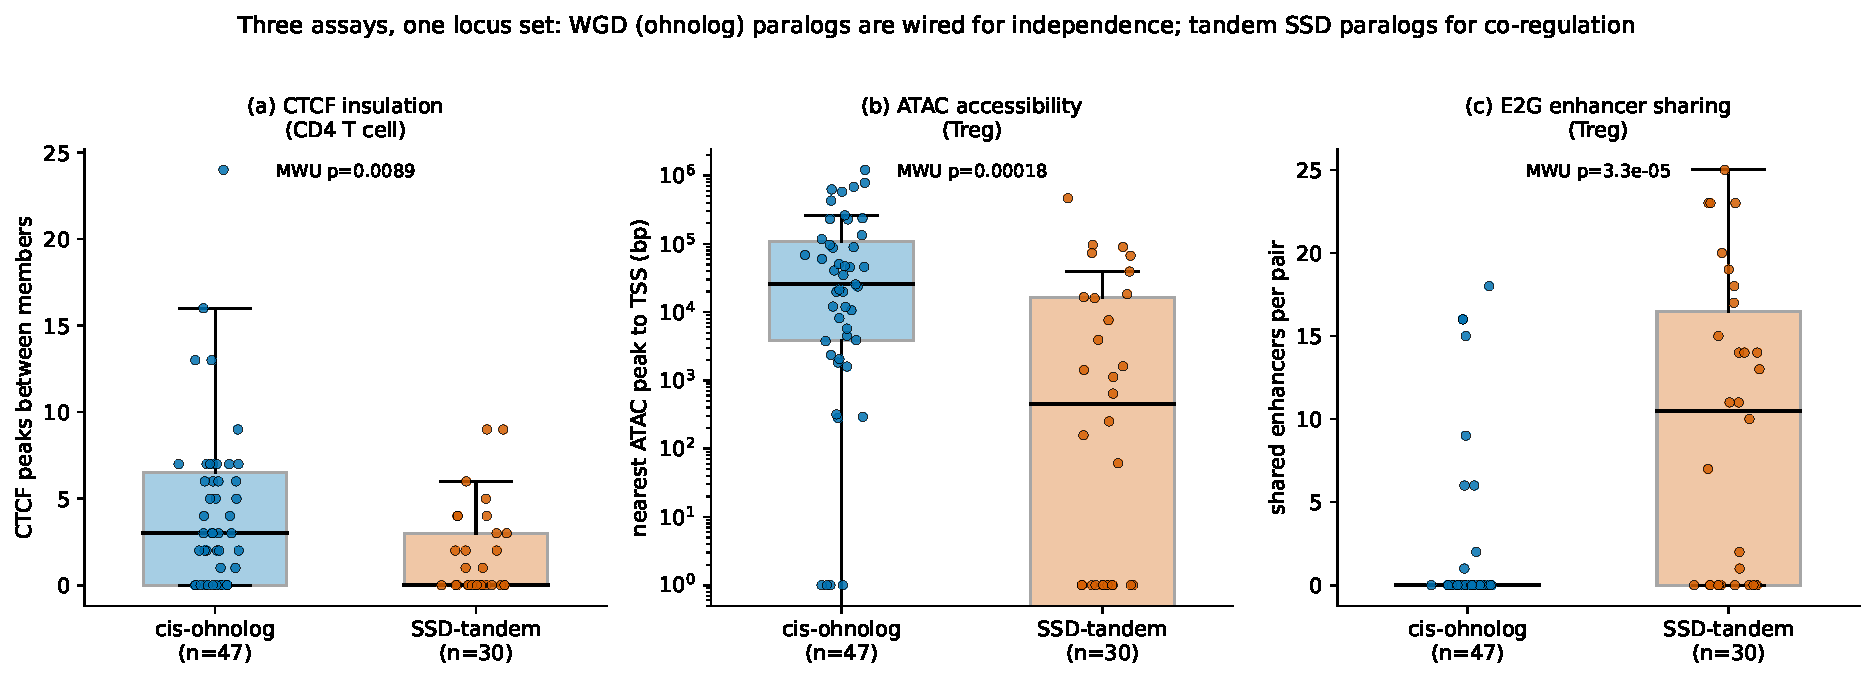
\includegraphics[width=\textwidth]{integrated_three_assay_headline.pdf}
\caption{Three assays, one locus set ($47$ \ohno{} blue, $30$ \ssd{} orange). (a) CTCF peaks between
the two paralog members (CD4 T cell); (b) distance from a member TSS to the nearest ATAC peak
(Treg; log axis); (c) enhancer elements shared by both paralogs (Treg E2G). Boxes = median/IQR,
points = loci, $p$ = Mann--Whitney~U.}
\label{fig:integrated}
\end{figure}

\begin{table}[H]
\centering
\caption{Cross-assay summary over the same 77 clustered loci (Mann--Whitney~U, \ohno{} vs.\ \ssd{};
\texttt{results/integrated\_cross\_assay\_summary.tsv}).}
\label{tab:integrated}
\small
\begin{tabular}{llccc}
\toprule
Assay (layer) & Headline metric & median (ohno) & median (SSD) & $p$ \\
\midrule
CTCF --- insulation (CD4 T) & CTCF peaks between the two members & 3 & 0 & $8.9\times10^{-3}$ \\
ATAC --- accessibility (Treg) & Nearest ATAC peak to member TSS (bp) & 25{,}492 & 446 & $1.8\times10^{-4}$ \\
E2G --- wiring (Treg) & Enhancers shared by both paralogs & 0 & 10.5 & $3.3\times10^{-5}$ \\
\bottomrule
\end{tabular}
\end{table}

\subsection{CTCF insulation: bulk density is equal; only between-member counts differ}
Both clustered groups are CTCF-enriched over the genome-wide expectation (observed/expected
$\sim$1.5--2.1$\times$), and bulk CTCF density across the $\pm$100~kb window is statistically
indistinguishable between them in both cell types (Table~\ref{tab:ctcf}; all $p>0.7$ for peaks/kb
window, body and flanks). The one metric that separates the groups is the \emph{number of CTCF peaks
between the two paralog members}: median $3$ (ohnolog) vs.\ $1$ (SSD) in GM12878 ($p=3.5\times10^{-3}$)
and $3$ vs.\ $0$ in CD4 T cells ($p=8.9\times10^{-3}$). However, ohnolog members are also farther
apart (median inter-member TSS distance $74$~kb vs.\ $49$~kb), and once the between-member CTCF count
is normalized to that distance the difference is no longer significant ($p=0.27$ GM12878, $p=0.067$
CD4). In other words, ohnolog pairs are separated by \emph{more} insulator elements because they span
\emph{more} DNA, not because the intervening chromatin is intrinsically denser in CTCF. CTCF thus does
not, on its own, distinguish the two duplication modes --- the distinction emerges only in the
accessibility and enhancer-wiring layers below.

\begin{table}[H]
\centering
\caption{CTCF architecture, \ohno{} vs.\ \ssd{} (Mann--Whitney~U, two-sided; $n=47$ vs.\ $30$ loci),
in two cell types. ``between members'' = CTCF peaks strictly between the outermost member TSSs.}
\label{tab:ctcf}
\small
\begin{tabular}{lcccccc}
\toprule
& \multicolumn{3}{c}{GM12878 (constitutive)} & \multicolumn{3}{c}{CD4 T cell (matched)} \\
\cmidrule(lr){2-4}\cmidrule(lr){5-7}
Metric & med (ohno) & med (SSD) & $p$ & med (ohno) & med (SSD) & $p$ \\
\midrule
CTCF peaks/kb (window)          & 0.025 & 0.022 & 0.92  & 0.026 & 0.027 & 0.89 \\
Observed/expected CTCF (window) & 1.70  & 1.52  & 0.92  & 1.96  & 2.05  & 0.89 \\
CTCF peaks between members      & 3.0   & 1.0   & $3.5\times10^{-3}$ & 3.0 & 0.0 & $8.9\times10^{-3}$ \\
\ldots normalized to distance   & 0.023 & 0.018 & 0.27  & 0.019 & 0.0   & 0.067 \\
\bottomrule
\end{tabular}
\end{table}

\subsection{ATAC accessibility: SSD-tandem promoters are more accessible}
Across the $\pm$100~kb window, \ssd{} loci are more accessible than \ohno{} loci
(observed/expected ATAC $2.58$ vs.\ $1.19$; Mann--Whitney~U $p=0.016$), with the effect
concentrated in the locus body (ATAC peaks/kb $0.067$ vs.\ $0.019$; $p=0.010$). The sharpest
separation is at the promoters themselves: the mean distance from a member TSS to its nearest ATAC
peak is $446$~bp for SSD-tandem members versus $25{,}492$~bp for ohnolog members
(Mann--Whitney~U $p=1.8\times10^{-4}$, rank-biserial $-0.51$; Table~\ref{tab:atac}). In other words,
SSD-tandem paralog promoters sit essentially on top of an open-chromatin peak, while ohnolog
paralog promoters are, on average, tens of kb from the nearest ATAC peak. The number of ATAC peaks
lying \emph{between} the two promoters does not differ ($p=0.68$).

\begin{table}[H]
\centering
\caption{ATAC-seq accessibility, \ohno{} vs.\ \ssd{} (Treg, \texttt{ENCFF519QMA};
Mann--Whitney~U, two-sided; $n=47$ vs.\ $30$ loci).}
\label{tab:atac}
\small
\begin{tabular}{lcccc}
\toprule
Metric & median (ohnolog) & median (SSD) & $p$ & rank-biserial \\
\midrule
ATAC peaks/kb (window)              & 0.022 & 0.048 & 0.016 & $+0.33$ \\
ATAC peaks/kb (locus body)          & 0.019 & 0.067 & 0.010 & $+0.35$ \\
Observed/expected ATAC (window)     & 1.19  & 2.58  & 0.016 & $+0.33$ \\
Nearest ATAC peak to member TSS (bp, mean) & 25{,}492 & 446 & $1.8\times10^{-4}$ & $-0.51$ \\
ATAC peaks between the two promoters       & 2.0 & 2.5 & 0.68 & $+0.06$ \\
\bottomrule
\end{tabular}
\end{table}

\subsection{E2G: SSD-tandem paralogs share enhancers; ohnologs do not}
The ENCODE-rE2G enhancer$\rightarrow$gene links reveal the wiring behind the accessibility
difference (Table~\ref{tab:e2g}). \ssd{} pairs receive denser regulatory input on their promoters
(median $32.5$ links vs.\ $9$; $p=2.7\times10^{-4}$; $22.5$ vs.\ $9$ distinct enhancer elements;
$p=1.0\times10^{-3}$). The most striking difference is \emph{enhancer sharing}: a median of $10.5$
enhancer elements are predicted to regulate \emph{both} SSD-tandem paralogs, versus $0$ for ohnolog
pairs (Mann--Whitney~U $p=3.3\times10^{-5}$, rank-biserial $+0.49$; Fig.~\ref{fig:e2g}b). Expressed
as a fraction of the pair's total enhancer complement, half of the enhancers of an SSD-tandem pair
are shared (shared fraction median $0.50$ vs.\ $0$; $p=1.2\times10^{-3}$), and $63\%$ of SSD-tandem
pairs share at least one enhancer versus $19\%$ of ohnolog pairs. Restricting to enhancers physically
inside the $\pm$100~kb window preserves the effect (median $6$ vs.\ $0$ shared; $p=7.7\times10^{-5}$).
Per-element accessibility (\texttt{Open}) is similar between groups ($p=0.35$), so the difference is
in \emph{how many} elements are shared, not in how open each one is.

\begin{table}[H]
\centering
\caption{ENCODE-rE2G enhancer--gene wiring, \ohno{} vs.\ \ssd{} (Treg, \texttt{ENCFF393GIF};
Mann--Whitney~U, two-sided).}
\label{tab:e2g}
\small
\begin{tabular}{lcccc}
\toprule
Metric & median (ohnolog) & median (SSD) & $p$ & rank-biserial \\
\midrule
E2G elements/kb (window)                 & 0.030 & 0.066 & $5.5\times10^{-3}$ & $+0.38$ \\
E2G observed/expected (window)           & 0.97  & 2.14  & $5.5\times10^{-3}$ & $+0.38$ \\
E2G links to pair promoters (total)      & 9.0   & 32.5  & $2.7\times10^{-4}$ & $+0.49$ \\
Distinct enhancer elements on promoters  & 9.0   & 22.5  & $1.0\times10^{-3}$ & $+0.44$ \\
Shared enhancers (both paralogs)         & 0.0   & 10.5  & $3.3\times10^{-5}$ & $+0.49$ \\
Shared enhancers within $\pm$100~kb      & 0.0   & 6.0   & $7.7\times10^{-5}$ & $+0.46$ \\
Shared-enhancer fraction                 & 0.0   & 0.50  & $1.2\times10^{-3}$ & $+0.51$ \\
Mean enhancer accessibility (\texttt{Open}) & 9.37 & 10.00 & 0.35 & $+0.16$ \\
\bottomrule
\end{tabular}
\end{table}

\begin{figure}[H]
\centering

\includegraphics[width=0.32\textwidth]{e2g/e2g_element_density_by_group.pdf}\hfill

\includegraphics[width=0.32\textwidth]{e2g/e2g_shared_enhancers_by_group.pdf}\hfill

\includegraphics[width=0.32\textwidth]{e2g/e2g_promoter_links_by_group.pdf}
\caption{ENCODE-rE2G, \ohno{} (blue) vs.\ \ssd{} (orange). (a) Per-locus E2G element density in the
$\pm$100~kb window. (b) Enhancer elements shared by \emph{both} paralogs of a pair --- the headline
result. (c) Distinct E2G enhancer elements landing on the pair's promoters. Boxes show the median and
IQR; points are individual loci; $p$-values are Mann--Whitney~U.}
\label{fig:e2g}
\end{figure}

\begin{figure}[H]
\centering
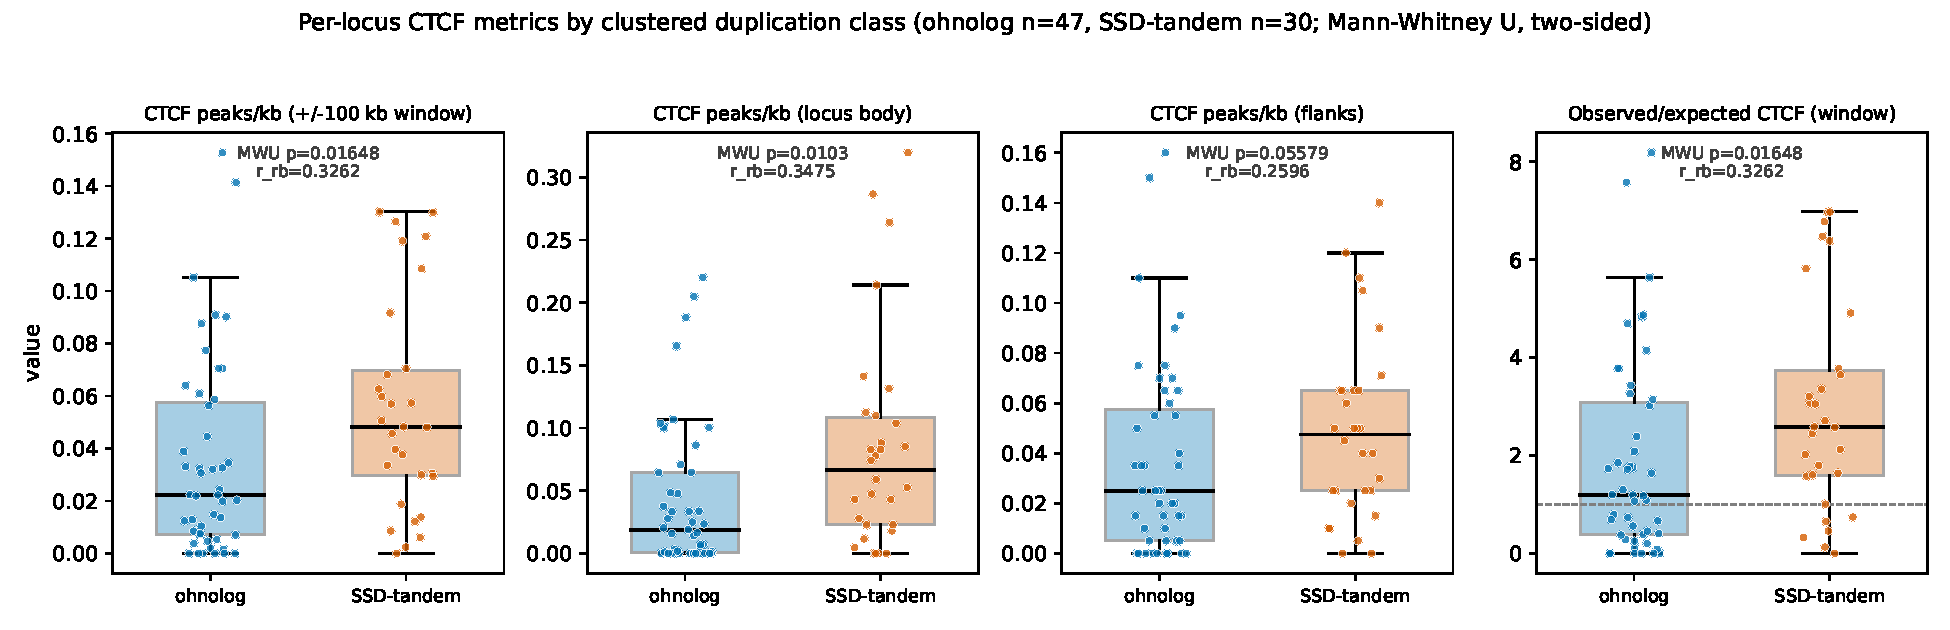
\includegraphics[width=0.42\textwidth]{atac/ctcf_peaks_per_kb_by_group.pdf}\hfill
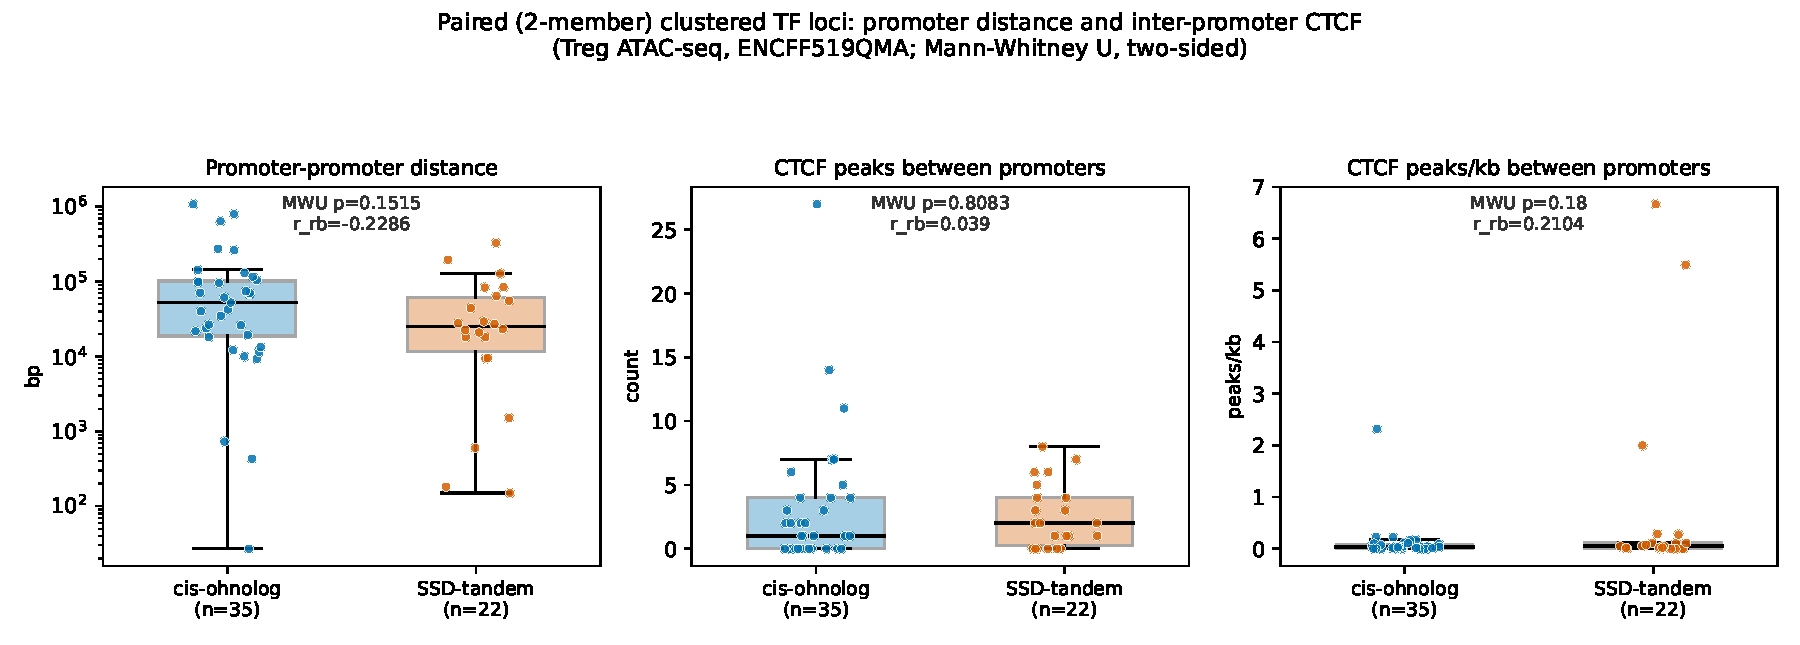
\includegraphics[width=0.42\textwidth]{atac/paired_promoters_ctcf.pdf}
\caption{ATAC-seq (Treg, \texttt{ENCFF519QMA}). Left: per-locus ATAC accessibility (peaks/kb) by
group. Right: paired-promoter ATAC summary. (Figures generated by the reused CTCF scripts under the
\texttt{atac} subdir; axis label ``CTCF'' in the shared script denotes ATAC peaks here.)}
\label{fig:atac}
\end{figure}

\subsection{Reproducibility across a 6-cell-type lymphoid panel}
To test whether the enhancer-sharing signature is specific to Treg, we re-ran the E2G analysis
on five additional ATAC-based ENCODE-rE2G sets (same extended model, hg38). ENCODE's ATAC-based
rE2G resource contains only three T-cell subtypes beyond Treg (memory CD4 \texttt{ENCFF440AKC},
CD8 \texttt{ENCFF993UOE}, and the T-ALL line Jurkat \texttt{ENCFF705FWU}); we added natural-killer
(\texttt{ENCFF359ZSL}) and B cells (\texttt{ENCFF186ABX}) as lymphoid controls. The result
reproduces in \emph{every} cell type (Table~\ref{tab:repro}, Fig.~\ref{fig:repro}): the median
number of enhancers shared by both paralogs is \textbf{0 for ohnolog pairs in all six cell types}
versus $6$--$10.5$ for SSD-tandem pairs, with Mann--Whitney~U $p$ ranging from $1.7\times10^{-5}$
(B cell) to $4.4\times10^{-3}$ (Jurkat, the leukemic line, is the weakest but still significant).
The per-locus obs/exp E2G density difference (SSD $>$ ohnolog) likewise reproduces in all
non-leukemic sets ($p\leq0.03$). The signature is therefore a robust property of the paralog
loci, not an artifact of one cell type.

\begin{table}[H]
\centering
\caption{Reproducibility of the shared-enhancer result across six lymphoid cell types
(ATAC-based ENCODE-rE2G; Mann--Whitney~U, two-sided, \ohno{} vs.\ \ssd{}; medians = shared
enhancers per pair). Bona-fide T cells in the top block; lymphoid controls below.}
\label{tab:repro}
\small
\begin{tabular}{llcccc}
\toprule
Cell type & file & median (ohnolog) & median (SSD) & $p$ & rank-biserial \\
\midrule
Treg              & ENCFF393GIF & 0 & 10.5 & $3.3\times10^{-5}$ & $+0.49$ \\
memory CD4 T      & ENCFF440AKC & 0 & 7.5  & $3.9\times10^{-5}$ & $+0.47$ \\
CD8 T             & ENCFF993UOE & 0 & 10.5 & $2.5\times10^{-4}$ & $+0.43$ \\
Jurkat (T-ALL)    & ENCFF705FWU & 0 & 7.0  & $4.4\times10^{-3}$ & $+0.35$ \\
\midrule
NK (control)      & ENCFF359ZSL & 0 & 6.0  & $1.1\times10^{-3}$ & $+0.38$ \\
B cell (control)  & ENCFF186ABX & 0 & 9.5  & $1.7\times10^{-5}$ & $+0.51$ \\
\bottomrule
\end{tabular}
\end{table}

\begin{figure}[H]
\centering
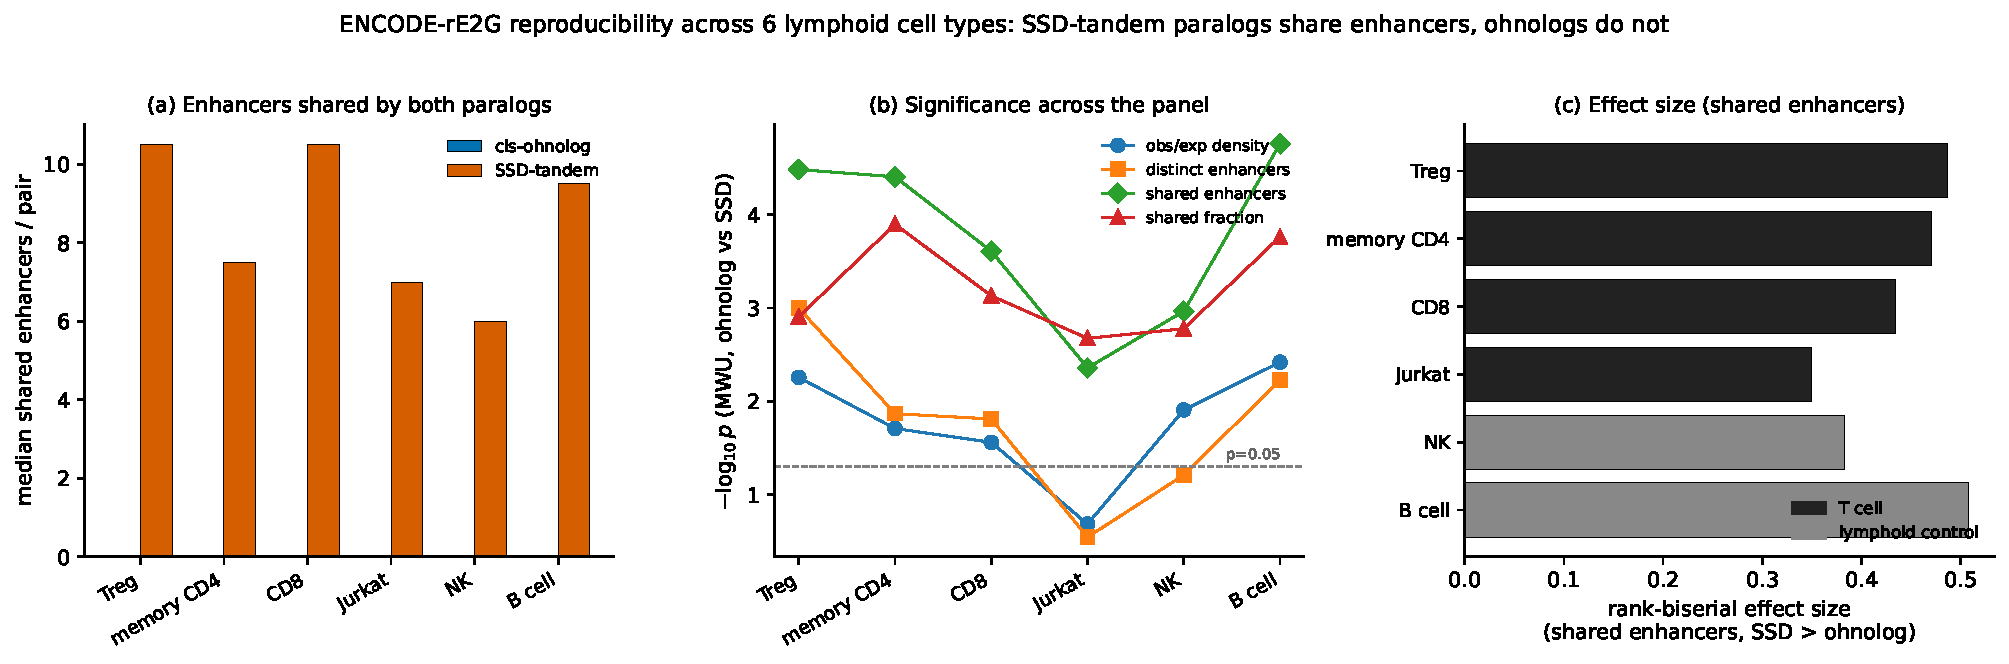
\includegraphics[width=\textwidth]{e2g/e2g_reproducibility.pdf}
\caption{ENCODE-rE2G reproducibility across six lymphoid cell types. (a) Median enhancers shared
by both paralogs, \ohno{} (blue) vs.\ \ssd{} (orange) --- ohnolog is $0$ everywhere. (b)
$-\log_{10}p$ (Mann--Whitney~U) for four E2G metrics across the panel; dashed line $p=0.05$.
(c) Rank-biserial effect size for the shared-enhancer test; dark bars = T cells, grey = lymphoid
controls.}
\label{fig:repro}
\end{figure}

\section{Interpretation}
The three assays layer into one coherent picture. The two clustered groups do \emph{not} differ in
their bulk insulator (CTCF) density --- CTCF alone cannot tell a WGD cluster from an SSD tandem
cluster, and the apparent between-member difference is a spacing artifact. The distinction lives
entirely in the accessibility and wiring layers. Tandem SSD paralogs --- recently duplicated and
physically adjacent --- occupy a single, highly accessible regulatory neighbourhood and are
co-regulated by a shared enhancer repertoire; roughly half of a tandem pair's enhancers act on both
genes. Cis-ohnolog paralogs, despite also being ``clustered'', retain sparser and more
\emph{independent} enhancer wiring, with promoters that are frequently far from the nearest
accessible peak, and (being farther apart) are separated by more insulator elements.
Together the picture is that WGD-derived clustered paralogs are wired for regulatory
\emph{independence} (insulated, sparse, unshared enhancers), whereas SSD tandem paralogs are wired
for \emph{co-regulation} (open, shared enhancers). For the ETS/P01 dosage-buffering thesis this is
directly relevant: shared-enhancer co-regulation predicts \emph{correlated} dosage between tandem
paralogs (a lesion in the shared enhancer would move both), while independent wiring predicts that
ohnolog paralogs can be dialed separately --- the substrate for paralog buffering.

\section{Caveats}
(i) Accessibility and enhancer--gene wiring are cell-type specific (Treg here, with CTCF from
GM12878 and resting CD4 T cells), unlike largely constitutive CTCF. (ii) ENCODE-rE2G links are model predictions (multiomic ABC-style), so
``shared enhancer'' counts depend on the score threshold baked into the released file. (iii) The two
groups are small ($n=47$ vs.\ $30$ loci); tests are reported at the locus level. (iv) Some cluster
members are readthrough / non-standard symbols that do not match a \texttt{TargetGene} and therefore
contribute zero links --- a conservative bias against detecting wiring. (v) Extended windows can
overlap for nearby clusters and were clipped to chromosome bounds.

\vspace{1em}
\noindent\small\textbf{Files.} CTCF: \texttt{results/ctcf/} (GM12878), \texttt{results/ctcf/cd4/};
ATAC: \texttt{results/ctcf/atac/}; E2G: \texttt{results/e2g/} (+ per-cell-type subdirs);
integration: \texttt{results/integrated\_cross\_assay\_summary.tsv},
\texttt{results/figures/integrated\_three\_assay\_headline.pdf}; figures under
\texttt{results/figures/\{atac,e2g\}/}; scripts \texttt{03--09}; logs in \texttt{log/}.

\end{document}
